\documentclass[hidelinks,11pt,dvipsnames]{article}
% xcolor commonly causes option clashes, this fixes that
\PassOptionsToPackage{dvipsnames,table}{xcolor}
\usepackage[tmargin=1in, bmargin=1in, lmargin=0.8in, rmargin=1in]{geometry}

%%%%%%%%%%%%%%%%%%%%%%%%%%%%%%%%%%%%%%%%%%%%%%%%%%%%%%%%%%%%%%%%%%%%
%%% For inkscape-figures
%%% Assumes the following directory structure:
%%% master.tex
%%% figures/
%%%     figure1.pdf_tex
%%%     figure1.svg
%%%     figure1.pdf
%%%%%%%%%%%%%%%%%%%%%%%%%%%%%%%%%%%%%%%%%%%%%%%%%%%%%%%%%%%%%%%%%%%%
%\usepackage{import}
\usepackage{pdfpages}
\usepackage{transparent}

\newcommand{\incfig}[2][1]{%
    \def\svgwidth{#1\columnwidth}
    \import{./figures/}{#2.pdf_tex}
}

\pdfsuppresswarningpagegroup=1

% enable synctex for inverse search, whatever synctex is
\synctex=1
\usepackage{float,macrosabound,homework,theorem-env}
\usepackage{microtype}


% font stuff
\usepackage{sectsty}
\allsectionsfont{\sffamily}
\linespread{1.1}

% bibtex stuff
\usepackage[backend=biber,style=alphabetic,sorting=anyt]{biblatex}
\addbibresource{main.bib}

% colored text shortcuts
\newcommand{\blue}[1]{\color{MidnightBlue}{#1}}
\newcommand{\red}[1]{\textcolor{Mahogany}{#1}}
\newcommand{\green}[1]{\textcolor{ForestGreen}{#1}}


% use mathptmx pkg while using default mathcal font
\DeclareMathAlphabet{\mathcal}{OMS}{cmsy}{m}{n}

% fixes the positioning of subscripts in $$ $$
\renewcommand{\det}{\operatorname{det}}

\usetikzlibrary{positioning, arrows.meta}
\newcommand{\here}[2]{\tikz[remember picture]{\node[inner sep=0](#2){#1}}}

%%%%%%%%%%%%%%%%%%%%%%%%%%%%%%%%%%%%%%%%%%%%%%%%%%%%%%%%%%%%%%%%%%%%%
%%% Entry Counter
%%%%%%%%%%%%%%%%%%%%%%%%%%%%%%%%%%%%%%%%%%%%%%%%%%%%%%%%%%%%%%%%%%%%%
\newcounter{entry-counter}
\newcommand{\entry}[1]
{
	\addtocounter{entry-counter}{1}
    \tchap{Entry \arabic{entry-counter}}
	%\addcontentsline{toc}{section}{Entry \arabic{entry-counter}: #1}
	\vspace{-1.5em}
    \begin{center}
		\small \emph{Written: #1}
    \end{center}
}

\usepackage{titling}
\renewcommand\maketitlehooka{\null\mbox{}\vfill}
\renewcommand\maketitlehookd{\vfill\null}


\usepackage{caption}
\usepackage{tikz}
\usetikzlibrary{positioning,calc,intersections,through,backgrounds, shapes.geometric, decorations.markings,arrows}

\def\sset{\subseteq}
\def\iso{\cong}
\def\gend#1{\langle #1\rangle}

\newcommand{\rightoverleftarrow}{%
  \mathrel{\vcenter{\mathsurround0pt
    \ialign{##\crcr
      \noalign{\nointerlineskip}$\longrightarrow$\crcr
      \noalign{\nointerlineskip}$\longleftarrow$\crcr
    }%
  }}%
}

\newcommand\makesphere{} % just for safety
\def\makesphere(#1)(#2)[#3][#4]{%
  % Synopsis
  % \makesphere[draw options](center)(initial angle:final angle:radius)
  \shade[ball color = #3, opacity = #4] #1 circle (#2);
  \draw #1 circle (#2);
  \draw ($#1 - (#2, 0)$) arc (180:360:#2 and 3*#2/10);
  \draw[dashed] ($#1 + (#2, 0)$) arc (0:180:#2 and 3*#2/10);
}
% same thing as makesphere but places white background behind
\newcommand\altmakesphere{} % just for safety
\def\altmakesphere(#1)(#2)(#3)[#4][#5]{%
  % Synopsis
  % \makesphere[draw options](center)(initial angle:final angle:radius)
  \draw [fill=white!30] #1 circle (#2);
  \shade[ball color = #4, opacity = #5] #1 circle (#2);
  \draw #1 circle (#2);
  \draw ($#1 - (#2, 0)$) arc (180:360:#2 and 3*#2/10);
  \draw[dashed] ($#1 + (#2, 0)$) arc (0:180:#2 and 3*#2/10);
  \node at #1 {#3};
}

\begin{document}
\pagestyle{empty}
	\LARGE
\begin{center}
	Algebraic Topology Homework 4 \\
	\Large
	Isaac Martin \\
    Last compiled \today
\end{center}
\normalsize
\vspace{-4mm}
\hru

\tchap{Problems from 1.2}

\begin{homework}[e]
  \prob[\textsc{Exercise 1.3}] Let $p:\tilX \to X$ be a covering space with $p^{-1}(x)$ finite and nonempty for all $x \in X$. Show that $\tilX$ is compact Hausdorff if and only if $X$ is compact Hausdorff.
  \begin{prf}
    First, a quick lemma.
    \begin{lem}
      Suppose $f:X\to Y$ is a local homeomorphism between topological spaces $X$ and $Y$, i.e. That at every point $x \in X$ there exists some open neighborhood $U\subseteq X$ of $x$ such that $f(U)$ is open and the restriction $f|_U$ is a homeomorphism onto $f(U)$. Then $f$ is an open map.
    \end{lem}
    \begin{proof}
      Let $U \subseteq X$ be an open set. Around each point $x \in V$ we may find an open set $U_x$ which maps homeomorphically to an open set $V_{x} = f(U_x)$ via $f$. Then $f(U_x\cap U)$ is open in $V_x$ equipped with the subspace topology. This means $f(U_x \cap U) = V_x \cap A$ for some open set $A \subseteq X$, but then $f(U_x\cap U)$ is a finite intersection of opens in $Y$ and hence itself open. We then have that
      \begin{align*}
        f(U) = \bigcup_{x\in U} f(U_x \cap U),
      \end{align*}
      and therefore $f(U)$ is open.
    \end{proof}

    Let's take care of Hausdorffness first. Suppose $X$ is Hausdorff and choose any two $x,y \in \tilX$ with $x \neq y$. There are two cases to consider depending on whether or not $x$ and $y$ lie in the same fiber. If they do not, then by Hausdorffness on $X$ we may find open neighborhoods $U \subseteq X$ for $p(x)$ and $V \subseteq X$ for $p(y)$ such that $U\cap V = \emptyset$. Then $p^{-1}(U)$ and $p^{-1}(V)$ are disjoint open neighborhoods of $x$ and $y$ respectively since $p$ is continuous. If instead $f(x) = f(y)$, take an open neighborhood $V\subseteq X$ of $f(x)$ which is evenly covered. Let $U$ and $U'$ be the open sets in the collection determined by $f^{-1}(V)$ which contain $x$ and $y$ respectively. Note that $x$ and $y$ are only contained in one such open set by the assumption that $f^{-1}(V)$ is a disjoint union of such sets. If $U = U'$, then the restriction $p|_U:U\to V$ would not be injective and hence could not be a homeomorphism. But $p|_U$ is a homeomorphism, hence $y\not\in U$ which implies $U$ and $U'$ are separating neighborhoods for $x$ and $y$. In either case, if $X$ is Hausdorff then $\tilX$ is Hausdorff.

    Now suppose that $\tilX$ is Hausdorff. Pick two distinct points $x,y\in X$ and let $U$ and $V$ be evenly covered neighborhoods of $x$ and $y$ respectively. Choose $\tilx \in f^{-1}(x), \tily \in f^{-1}(y)$, and let $\tilU$ and $\tilV$ be open sets mapping homeomorophically to $U$ and $V$ respectively via $p$ such that $\tilx \in \tilU$ and $\tily \in \tilV$. That is, pick $\tilx$, $\tily$, $\tilU$ and $\tilV$ to be points/open sets in $\tilX$ corresponding to $x,$ $y$, $U$ and $V$ in $X$ via $p$. Since $\tilX$ is Hausdorff, we may find separating neighborhoods $\tilA$ of $\tilx$ and $\tilB$ of $\tily$ such that $\tilA \cap \tilB = \emptyset$. Set $A = p(\tilU \cap \tilA)$ and $B = p(\tilV\cap \tilB)$. We have that $x \in A$ since $\tilx \in \tilU \cap \tilA$ and likewise $y \in B$. Because $p$ is a homeomorphism on $\tilU$, it is an open map and $A$ is therefore open in the subspace topology in $U$. This means there is some open set $U'$ such that $A = U\cap U'$ in $X$, implying that $A$ is open in $X$ since finite intersections of opens are open. The set $B\subseteq X$  is open by similar reasoning. Finally, if there were some $z \in A\cap B$, then there must be some $\tilz \in (\tilU \cap \tilA) \cap (\tilV \cap \tilB)$ since $p|_{\tilU \cap \tilV} \to U\cap V$ is a homeomorphism. There is no such $\tilz$ since $\tilA$ and $\tilB$ were chosen to be separating neighborhoods in $\tilX$, hence $A$ and $B$ are disjoint. This proves we can separate distinct points in $X$ by open sets, and hence $X$ is Hausdorff.

    \bigskip

    We now move on to compactness. One direction is easy: from pointset topology we know that the image of a compact set under a continuous map is compact, hence $X = p(\tilX)$ is compact if $\tilX$ is compact. To see this, take an open cover $\{U_\alpha\}_{\alpha \in A}$ of $X$. Then $\{p^{-1}(U_\alpha)\}_{\alpha \in A}$ is an open cover of $\tilX$ and must have a finite subcover $\{p^{-1}(U_1),...,p^{-1}(U_n)\}$. But then $\{pp^{-1}(U_1),...,pp^{-1}(U_n)\} = \{U_1,...,U_n\}$ is an open cover of $X$ by the surjectivity of $p$.

    Suppose now that $X$ is compact and choose some open cover $\cU$ of $X$. I first claim that for each $x \in X$, we may find an open neighborhood $V_x\subseteq X$ of $x$ such that each lift of $V_x$ is contained in $U_\alpha$ for some $\alpha$. The idea is to shrink an evenly covered neighborhood of $x$ until it satisfies the desired property. Indeed, since $f^{-1}(x) = \{\tilx_1,...,\tilx_n\}$ is finite, we may find $U_1,...,U_n$ such that $\tilx_i \in U_i$. By the definition of a covering space, we can find an evenly covered neighborhood $V\subseteq X$ of $x$. Since each lift of $V$ contains exactly one element of the fiber of $x$, there are exactly $n$-lifts of $V$, and we enumerate them $\tilV_1,...,\tilV_n$. Define the intersection $\tilW_i = \tilV_i \cap U_i$. Each $\tilW_i$ contains $\tilx_i$, and is hence a nonempty open set of $\tilX$. Furthermore, $W_i = p(\tilW_i)$ is a homeomorphic to $\tilW_i$ since the restriction of $p$ to $\tilV_i$ is a homeomorphism by definition. Now define $V_x = W_1\cap ...\cap W_n$. We have that $V_x$ is a neighborhood of $x$ since $\tilx_i \in \tilW_i \implies x = p(\tilx_i)\in W_i = p(\tilW_i)$ for each $i$ and each lift of $V_x$ is entirely contained in $\tilW_i \subseteq U_i$ for some $1\leq i\leq n$, proving the claim. 

    Choosing such a $V_x$ for each $x \in X$ gives us a cover $\cV$ of $X$, and hence by compactness we may find a finite subcover $\cV' = \{V_{x_1},...,V_{x_n}\}$. Because each $V_x$ was constructed above as a subset of an evenly covered neighborhood of $x$, it to is an evenly covered neighborhood of $x$ and hence has exactly $n$ lifts. This implies that the lift $\cV'$ to $\tilX$ is also a finite cover. For each $1\leq i\leq n$ and each lift $V_{x_i}$, there is some $U \in \cU$ containing that lift, and since we have finitely many lifts for each $V_{x_i}$ and finitely many $V_{x_i}$ in the collection $\cV'$, the lift of $\cV'$ to $\tilX$ has a refinement to a finite sub cover of $\cU$. This proves that $\tilX$ is compact.
  \end{prf} 

  \prob[\textsc{Exercise 1.4}] Construct a simply-connected covering space of the space $X\subseteq \bR^3$ that is the union of a sphere and a diameter. Do the same when $X$ is the union of a sphere and a circle intersecting it in two points.
  \begin{prf}
    Let $X\subseteq \bR^3$ be the union of unit sphere $S^2$ in $\bR^3$ with its diameter $D$ connecting its north and south poles on the $x$-axis, i.e. the line segment between $(-1,0,0)$ and $(1,0,0)$. Now for $t \in \bR$ let $T_t:\bR^3\to \bR^3$ be the homeomorphism of $\bR^3$ given by translating by $t$ along the $x$-axis, that is, $T_t(x,y,z) = (x+t,y,z)$.

    I claim that
    \begin{align*}
      \tilX = \bigcup_{n\in \bZ} (T_{4n}(S^2) \cup T_{4n+1}(D)),
    \end{align*}
    seen in Figure (\ref{fig:prob4-1}), is a simply-connected cover of $X$. By deformation retracting each $T_{4n+1}(D)$ to a point, we see that $\tilX$ is homotopy equivalent to an infinite wedge of spheres, and hence simply connected. To see that it is a covering space of $X$, we need to construct a covering map. Define $p:\tilX\to X$ to be the inverse translation $T_{-4n}$ on each sphere $T_{4n}(S^2)$ and the inverse translation $T_{-(4n+1)}$ followed by a reflection across the $yz$-plane on each line segment $T_{4n+1}(D)$. Then for each point $x \in X$ we can find an $\epsilon > 0$ small enough so that $p^{-1}(B_\epsilon(x)\cap X)$ is a union of disjoint homeomorphic copies of $B_\epsilon(x)\cap X$, each lift given by a translate or a reflection followed by a translate.
    \begin{center}
      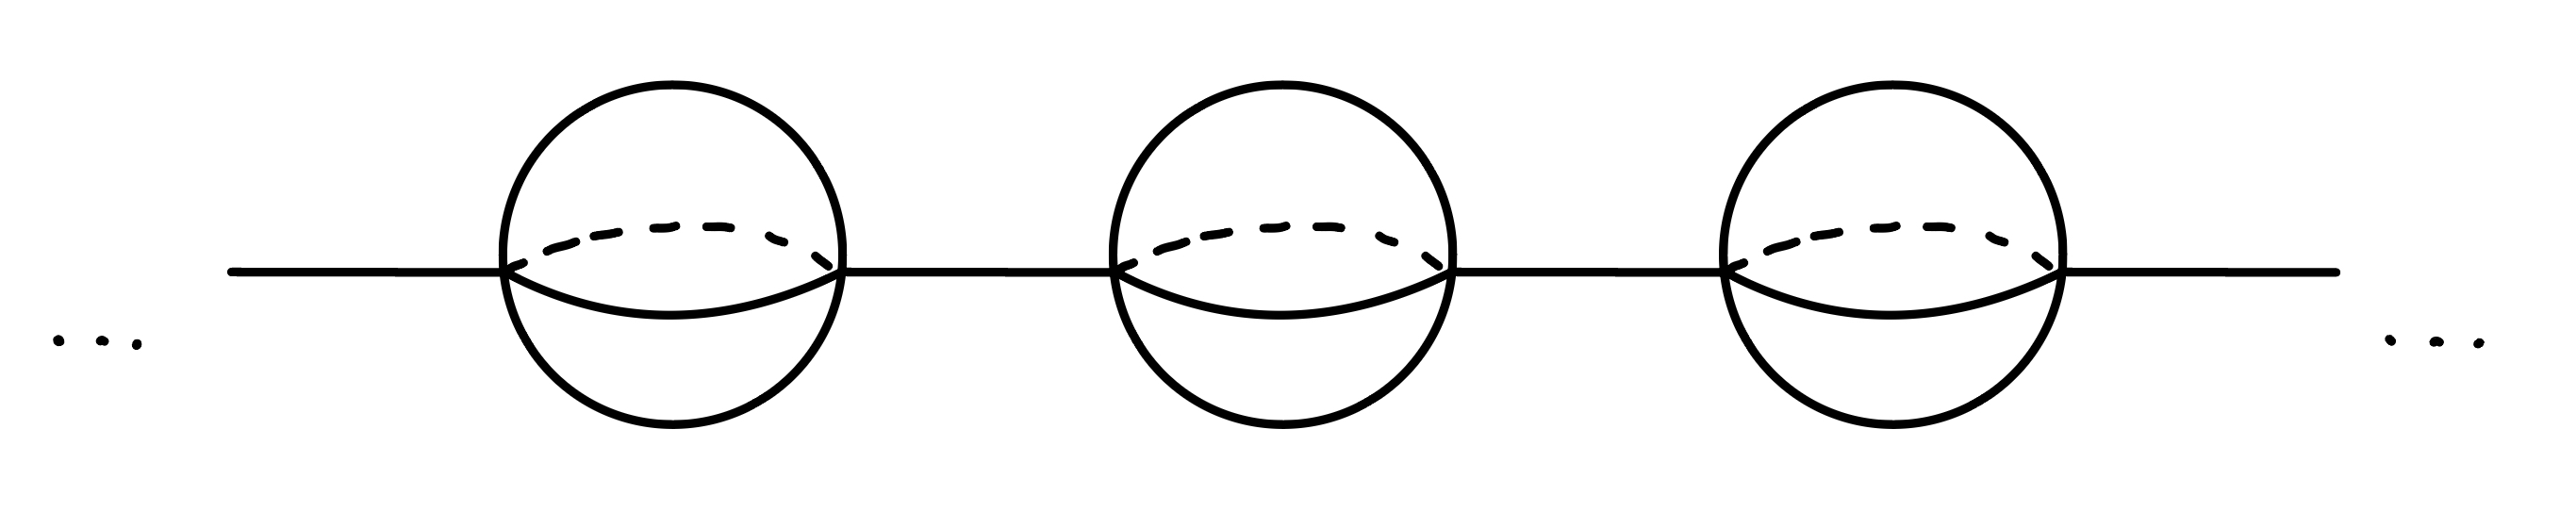
\includegraphics[width=10cm]{figures/hwk5-fig4.jpg}
      \captionof{figure}{Universal cover of the sphere union a diameter} 
      \label{fig:prob4-1}
    \end{center}

    Now let $X$ be the unit sphere $S^2$ in $\bR^3$ union a circle $S^1$ which intersects $S^2$ at exactly two points. By homotoping these two points along the section of the great arc connecting them on the surface of $S^2$, we see that $X$ is homotopy equivalent to $S^2 \vee S^1\vee S^1$ (see Figure \ref{fig:prob4-3}).

    For its universal cover, we first take the Cayley graph $Y$ from Example 1.45, the universal cover of $S^1\vee S^1$ equipped with covering map $p_1:Y\to S^1\vee S^1$. We then obtain a space $\tilX$ by wedging a copy of $S^2$ at every point of $p_1^{-1}(x)$, where $x$ denotes the basepoint of $S^1\vee S^1$. The space $\tilX$ is seen in Figure (\ref{fig:prob4-4}). The covering map $p:\tilX\to X$ sends each copy of $S^2$ to $S^2$ in $X$ and is defined to be $p_1$ on $Y$. The space $\tilX$ is simply connected since it is homotopy equivalent to the wedge of countably many spheres, again by the homotopy retracting each chord in $Y$ to a point.

    \begin{center}
      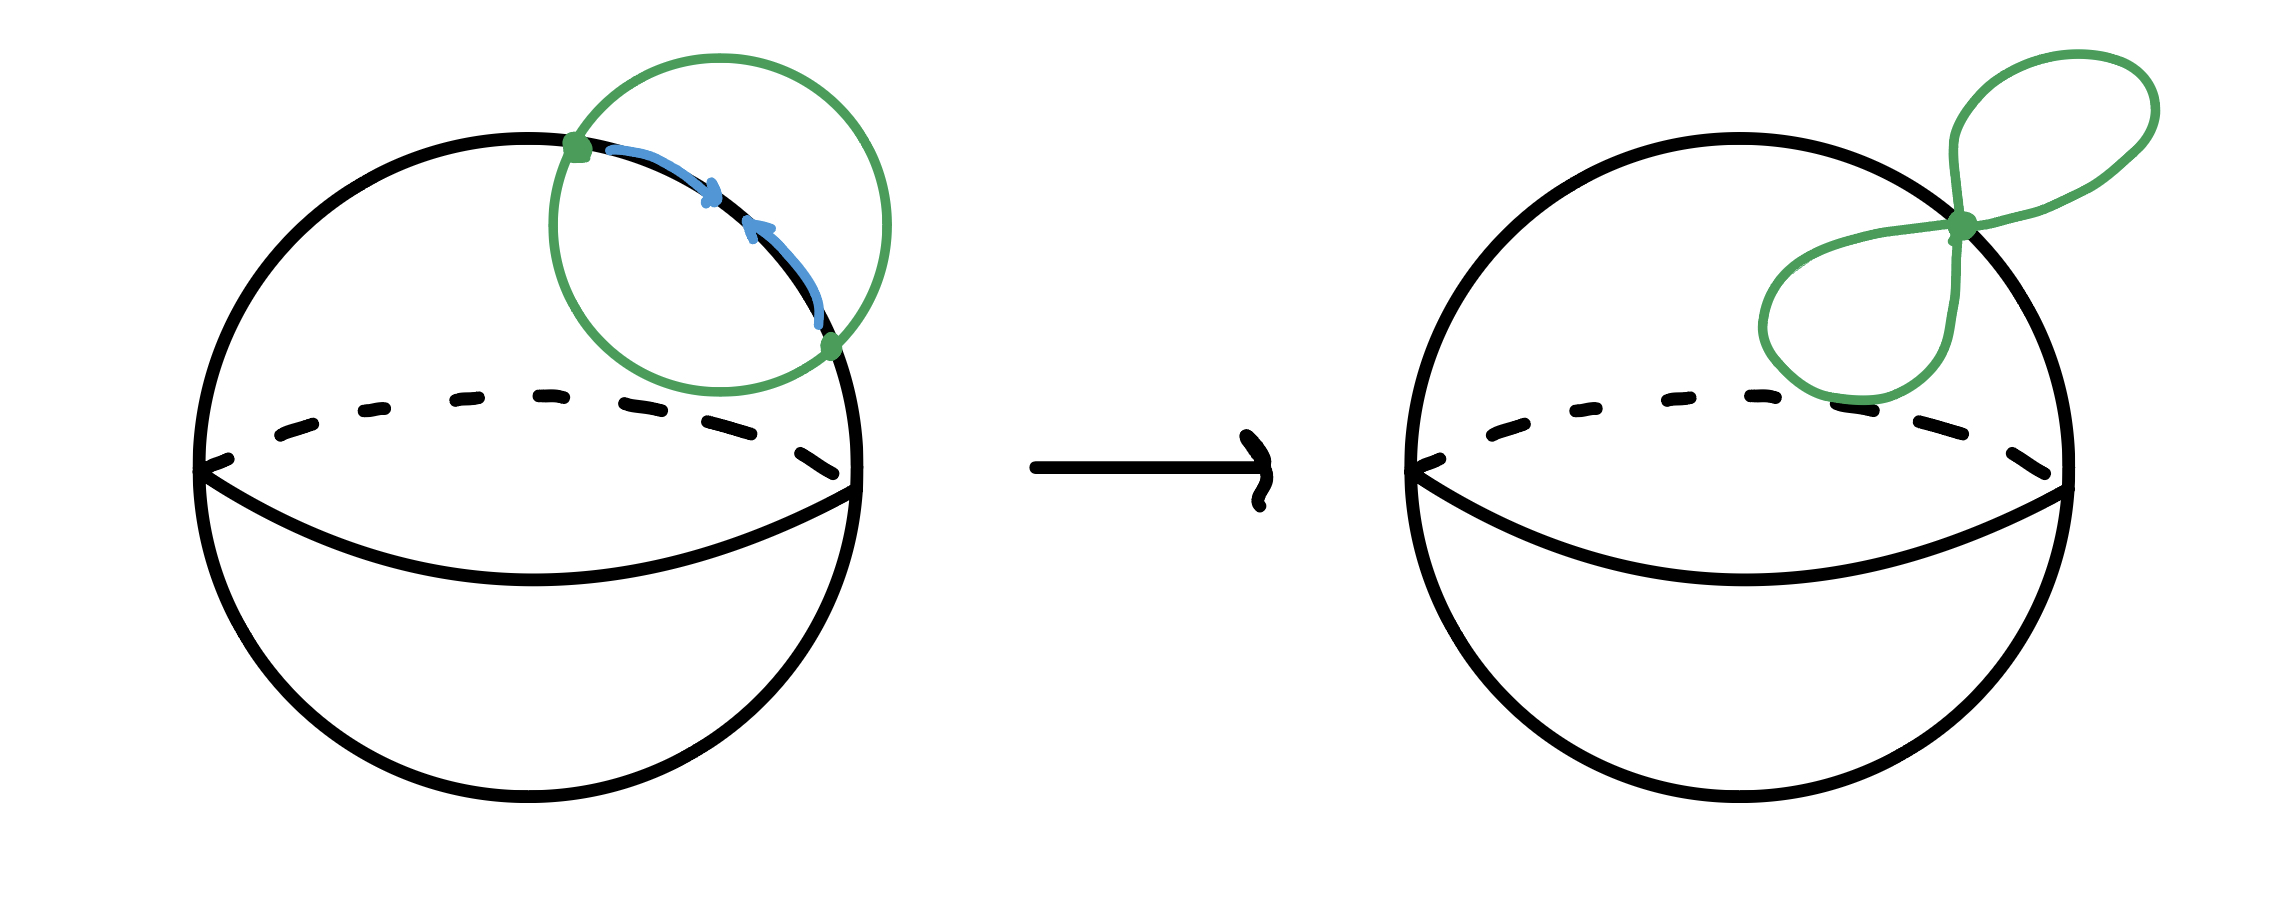
\includegraphics[width=10cm]{figures/hwk5-fig6.jpg}
      \captionof{figure}{The sphere union a circle intersecting it twice is homotopy equivalent to $S^2 \vee S^1 \vee S^1$} 
      \label{fig:prob4-3}
    \end{center}
    \begin{center}
      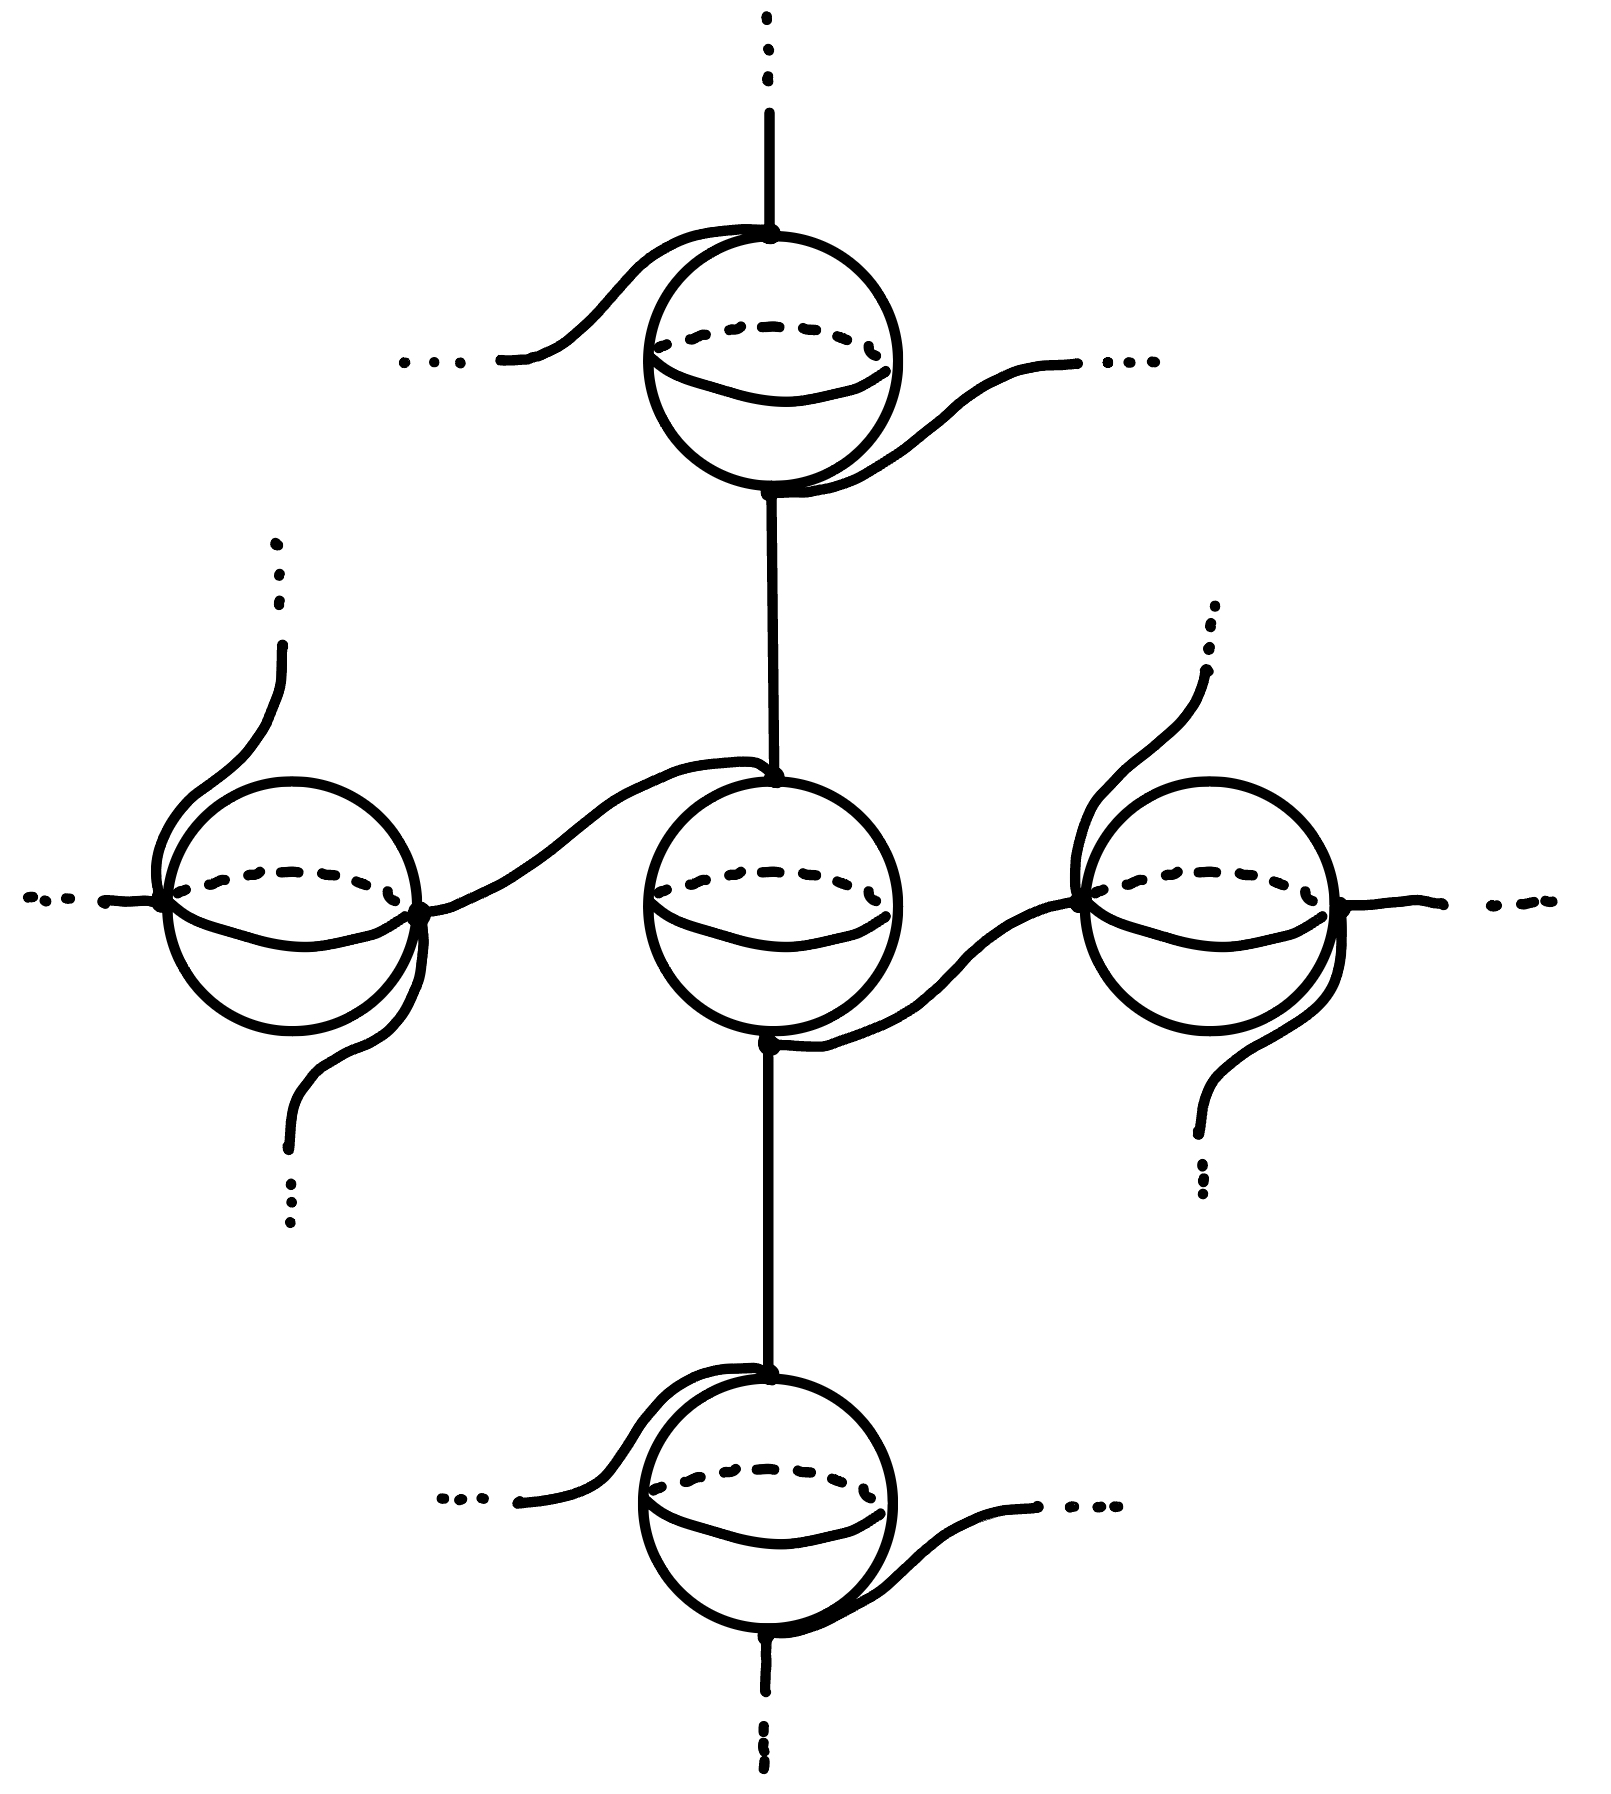
\includegraphics[width=10cm]{figures/hwk5-fig7.jpg}
      \captionof{figure}{The universal cover $\tilX$ of the sphere union a twice-intersecting circle.} 
      \label{fig:prob4-4}
    \end{center}
  \end{prf}
  \prob[\textsc{Exercise 1.5}] Let $X$ be the subspace of $\bR^2$ consisting of the four sides of the square $[0,1]\times [0,1]$ together with the segments of the vertical lines $x = \frac{1}{2},\frac{1}{3},\frac{1}{4},...$ inside the square. Show that for every covering space $\tilX\to X$ there is some neighborhood of the left edge of $X$ that lifts homeomorphically to $\tilX$. Deduce that $X$ has no simply-connected covering space. 
  \begin{prf}
    Call the leftmost edge of $X$ $E$. We first argue that if $\tilX$ is a covering space of $X$ then there is a neighborhood of $E$ that lifts homeomorphically to $\tilX$. By the definition of a covering space, for each point $x \in X$ there is some evenly covered neighborhood $U_x$ and the set of all such neighborhoods forms a cover for $X$. Closed and bounded in $\bR^2$ implies compact (Hein Borel baby) so there exists a finite subset $S\subseteq X$ such that $\{U_x\}_{x\in S}$ is a finite subcover of $X$. Define $T = \{x \in S ~\mid~ U_x \cap E \neq \emptyset\}$ and
    \begin{align*}
      U = \bigcup_{x\in T} U_x
    \end{align*}
    to be the union of all these evenly covered neighborhoods which intersect $E$ nontrivially. We argue that this set is an evenly covered neighborhood of $E$.

    Because $E$ is connected, there must be at least two distinct $x_1,x_2 \in T$ such that $U_{x_1}\cap U_{x_2} \neq \emptyset$. For any $y \in U_{x_1} \cap U_{x_2}$, let $V\subseteq U_{x_1} \cap U_{x_2}$ be an open neighborhood of $y$. Then $V$ is an evenly covered neighborhood of $y$, and each of its disjoint copies in $p^{-1}(U_{x_1})$ must intersect the corresponding copy in $p^{-1}(U_{x_2})$. This implies that $U_{x_1}\cup U_{x_2}$ is an evenly mapped neighborhood for both $x_1$ and $x_2$. By redefining $U_{x_1} = U_{x_1}\cup U_{x_2}$ and removing $x_2$ from $T$, we reduce the cardinality of $T$ by $1$ and leave $U$ unaffected, still covered by evenly covered sets. Since $T$ is finite, repeating this process must eventually terminate with $|T| = 1$, leaving us with only $U$, an evenly covered set containing $E$. This proves that $U$ is (one choice of) the desired neighborhood of $E$.

    Since $U$ is an open set in $X\subseteq \bR^2$ equipped with the subspace topology, there must be an open set $V \subseteq \bR^2$ such that $U = V\cap \bR^2$. Let $B$ denote the boundary of $V$, noting that it intersects $E$ trivially because $E\subseteq V$. Since $E$ is compact in $\bR^2$ and $E\cap B = \emptyset$, the minimum distance $r$ between $E$ and $B$ is attained by a pair of points in $E$ and $B$ and is positive. We can therefore find some $n\in \bN$ such that $\frac{1}{n}< r$. Since each point $x$ in the vertical line $L = \{1/n\}\times [0,1]$ of $X$ is distance $1/n$ from $E$, $x \in V$. This implies that $L\subseteq V$, and hence $L \subseteq U$. Likewise, each point along the horizontal segments $H_1$ and $H_2$ connecting $L$ to $E$ is within distance $1/n$ of $E$ and is hence also contained in U.

    The union $E \cup H_1\cup L\cup H_2$ lifts homeomorphically to $\tilX$ as it is contained in $U$, but this means that $\tilX$ contains a loop which is not nullhomotopic. We conclude that $\tilX$ is not simply connected, and since $\tilX$ was chosen to be an arbitrary cover space of $X$, that $X$ has no universal cover.

    \begin{center}
      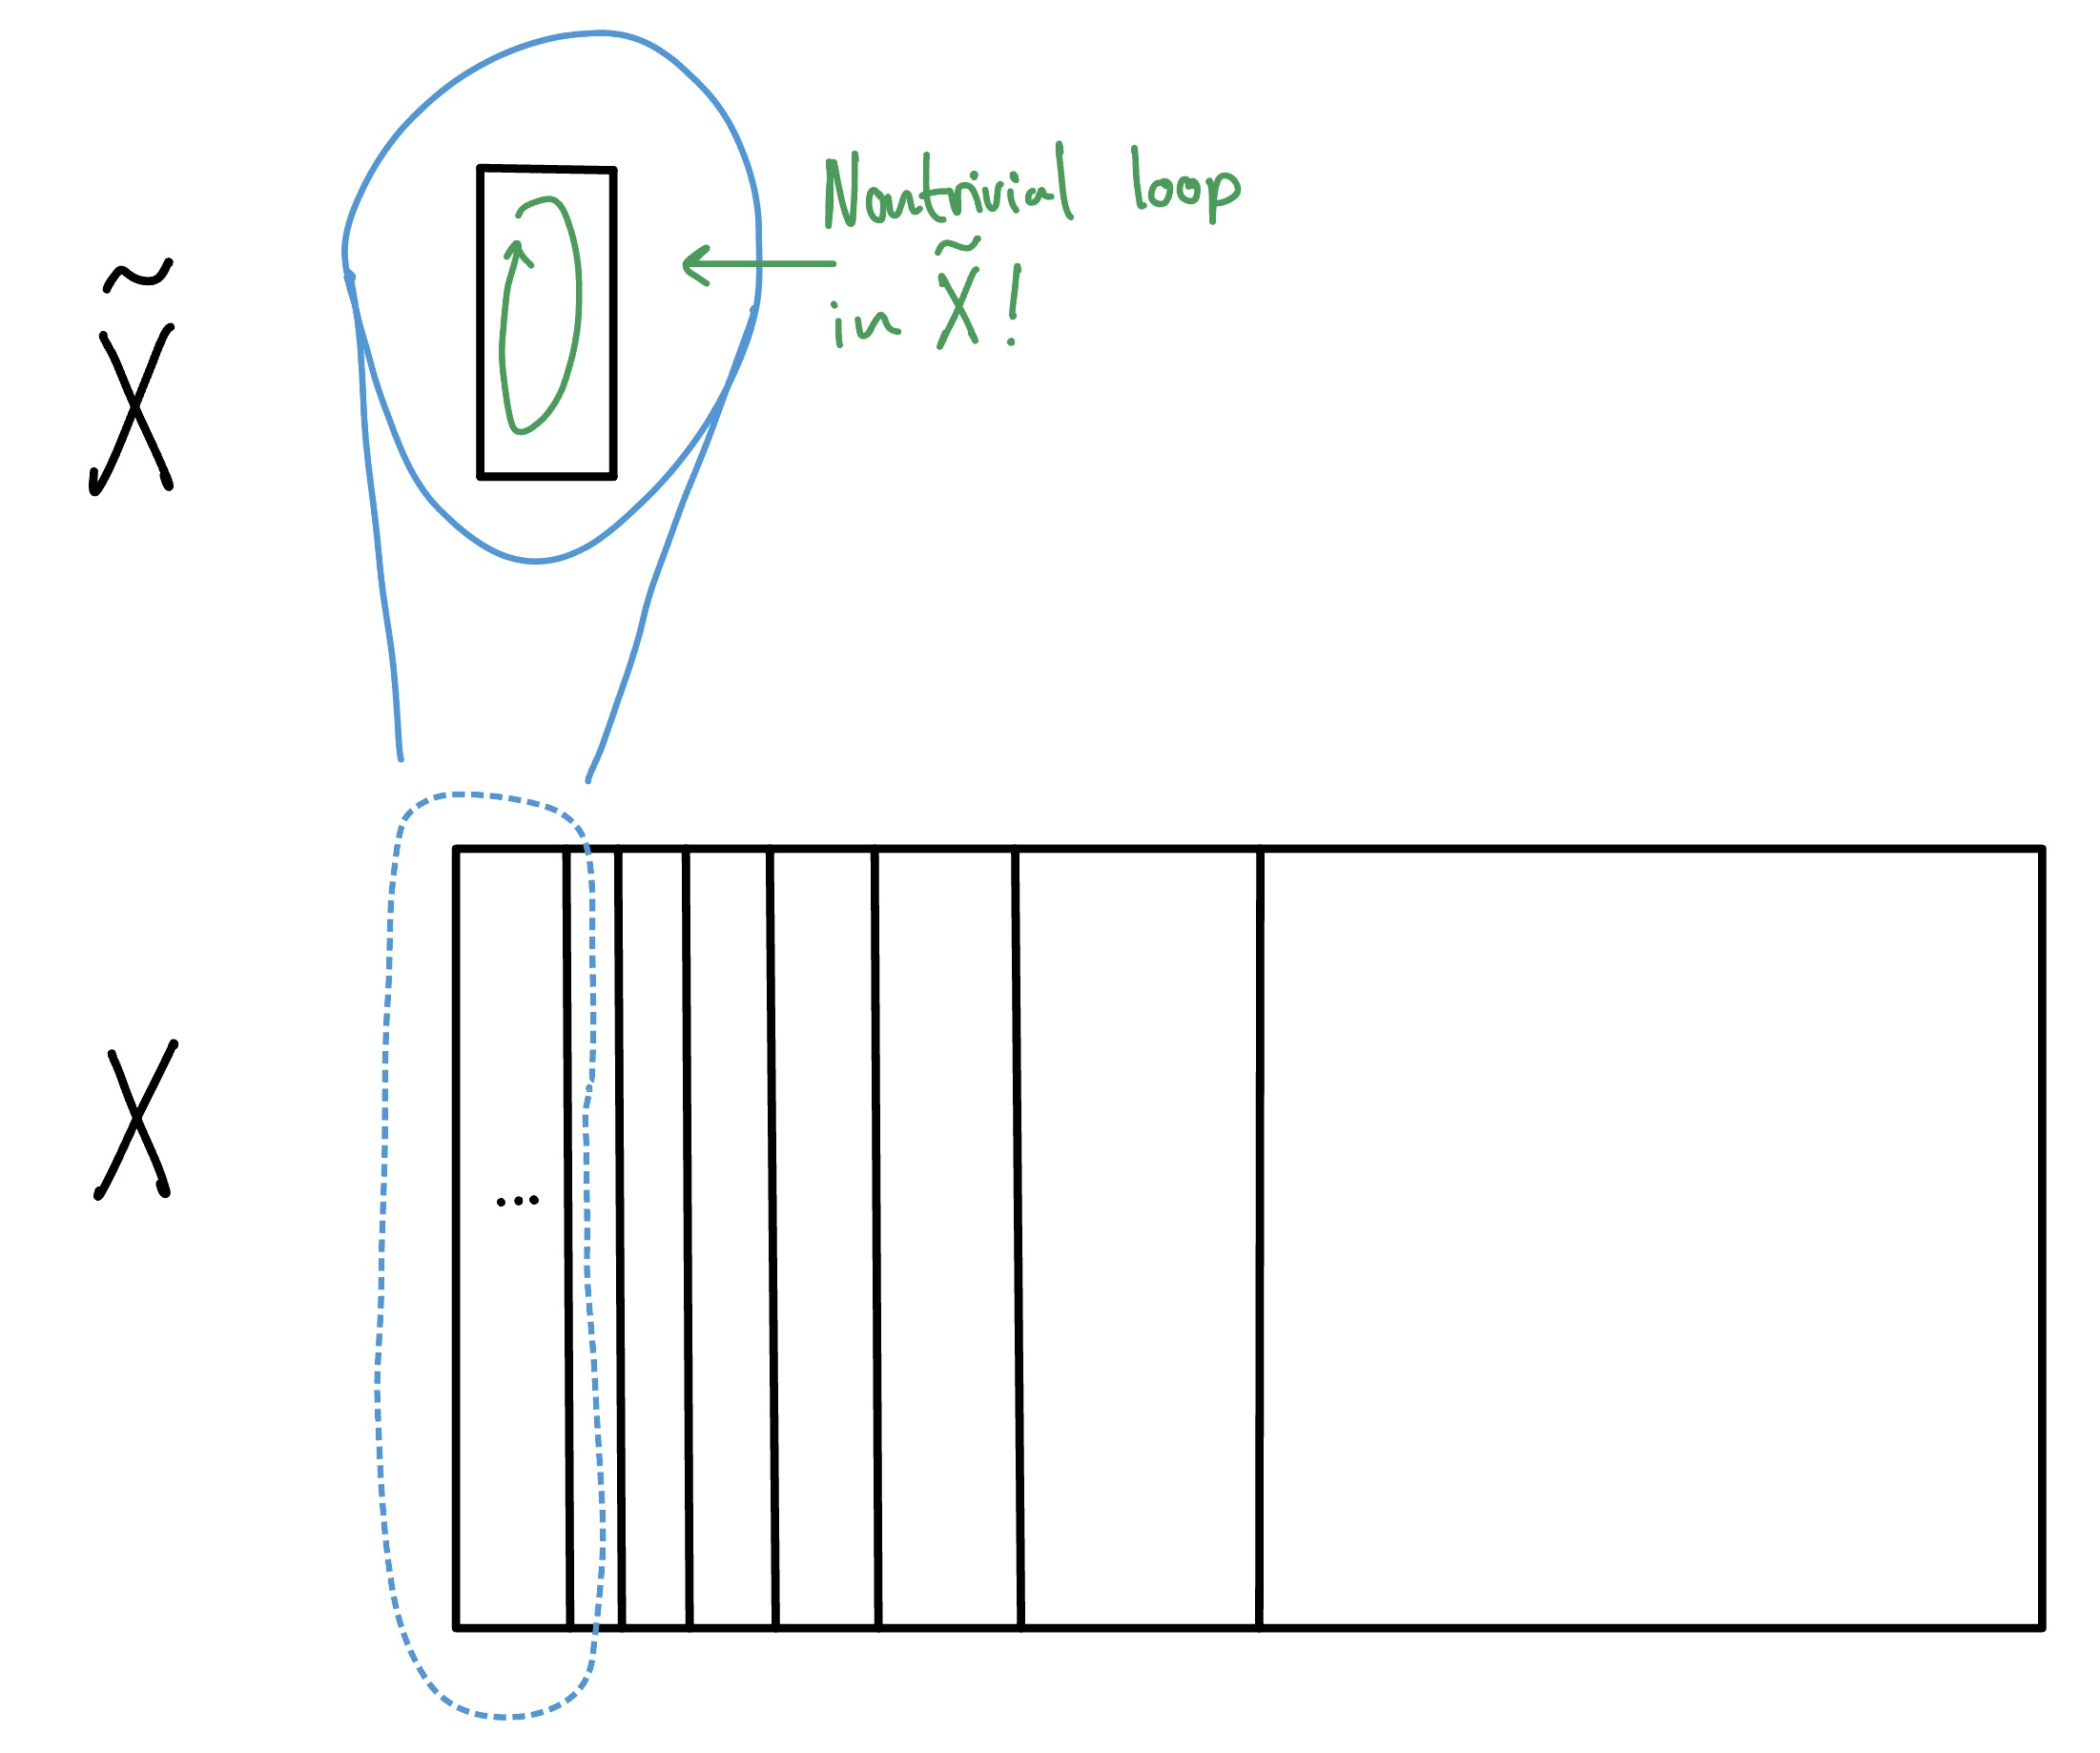
\includegraphics[width=10cm]{figures/hwk5-fig7.png}
      \captionof{figure}{$\tilX$ has a nontrivial loop.} 
      \label{fig:prob5-1}
    \end{center}
  \end{prf}
  \prob[\textsc{Exercise 1.9}] Show that if a path-connected, locally path-connected space $X$ has $\pi_1(X)$ finite, then every map $X\to S^1$ is nullhomotopic. [Use the covering space $\bR\to S^1$].
  \begin{prf}
    Note first that there is no finite subgroup of the additive group $\bZ$. Indeed, if $g \in \bZ$ were of finite order $k\geq 1$, then $k\cdot g = 0 \implies g = 0$ since $\bZ$ is an integral domain. The continuous map $f:X\to S^1$ induces a morphism $f_*:\pi_1(X,x_0)\to \pi_1(S^1,s_0)$, and since $\pi_1(X,x_0)$ is finite by assumption, this induced map must be the trivial map. This implies that $f_*(\pi_1(X,x_0)) = \langle 0 \rangle \subseteq p_*(\pi_1(\bR,r_0))$, where $p:\bR\to S^1$ is the covering map, and hence by the lifting criterion there exists a lift $\tilf:X\to \bR$ of $f$ sending $x_0$ to the arbitrarily chosen basepoint $r_0 \in \bR$. 

    Since $\bR$ deformation retracts to to $r_0$, $\tilf:X\to \bR$ is nullhomotopic to the constant map $g:X\to \bR$ defined $g(x) = r_0$. Let $\tilF:X\times [0,1]\to \bR$ be the homotopy taking $\tilf$ to $g$, i.e. a homotopy such that $\tilF(x,0) = \tilf(x)$ and $\tilF(x,1) = r_0$. Both $\tilF$ and $p$ are continuous, hence the composition $p\circ \tilF$ is continuous. But this is a homotopy taking $f$ to the constant map sending everything in $X$ to $s_0$, since $f = p\circ \tilf = p\circ \tilF(x,0)$ and $p\circ\tilF(x,1) = p(r_0) = s_0$. We conclude that $f:X\to S^1$ is nullhomotopic.
  \end{prf}
  \prob[\textsc{Exercise 1.12}] Let $a$ and $b$ be the generators of $\pi_1(S^1 \vee S^1)$ corresponding to the two $S^1$ summands. Draw a picture of the covering space of $S^1 \vee S^1$ corresponding to the normal subgroup generated by $a^2$, $b^2$ and $(ab)^4$, and prove that this covering space is indeed the correct one.
\begin{prf}
    The covering space corresponding to the subgroup normally generated by $a^2$, $b^2$ and $(ab)^4$ is seen in (\ref{fig:12_graph}). Call this space $\tilX$, set $X = S^1 \vee S^1$, and let $p: \tilX \rightarrow X$ be the covering map obtained by identifying all the $a$ edges and all the $b$ edges in $\tilX$. The $a$ and $b$ loops in $\tilX$ correspond to $a^2$ and $b^2$ respectively, while traversing the outer edges of the graph gives a loop corresponding to $(ab)^4$. To check that $\tilX$ does indeed correspond to the subgroups \emph{normally} generated by $a^2$, $b^2$ and $(ab)^4$, it suffices to check that $\tilX$ is a normal cover by Proposition 1.39. We therefore need to check that the group of deck transformations acts transitively on the fiber $p^{-1}(x)$ of the basepoint $x \in X$. 

    Let $\tilx$ be the orange point in the top left of the figure, near 11 o'clock. To move $\tilx$ clockwise around $\tilX$, we apply the deck transformations corresponding to $a$ and $b$ interchangably, starting with $a$. For example, applying $a$ takes $\tilx$ to the blue point near $1$ o'clock in the figure, $ab$ takes $\tilx$ to the orange point near 2 o'clock and so on. This procedure allows us to take $\tilx$ to any other point in $p^{-1}(x)$, and reversing this process can take any point in $p^{-1}(x)$ to $\tilx$. By passing through $\tilx$ we can take any point in $p^{-1}(x)$ to any other point, hence the action of deck transformations on $\tilX$ is transitive and $\tilX$ is a normal cover.
    \begin{center}
      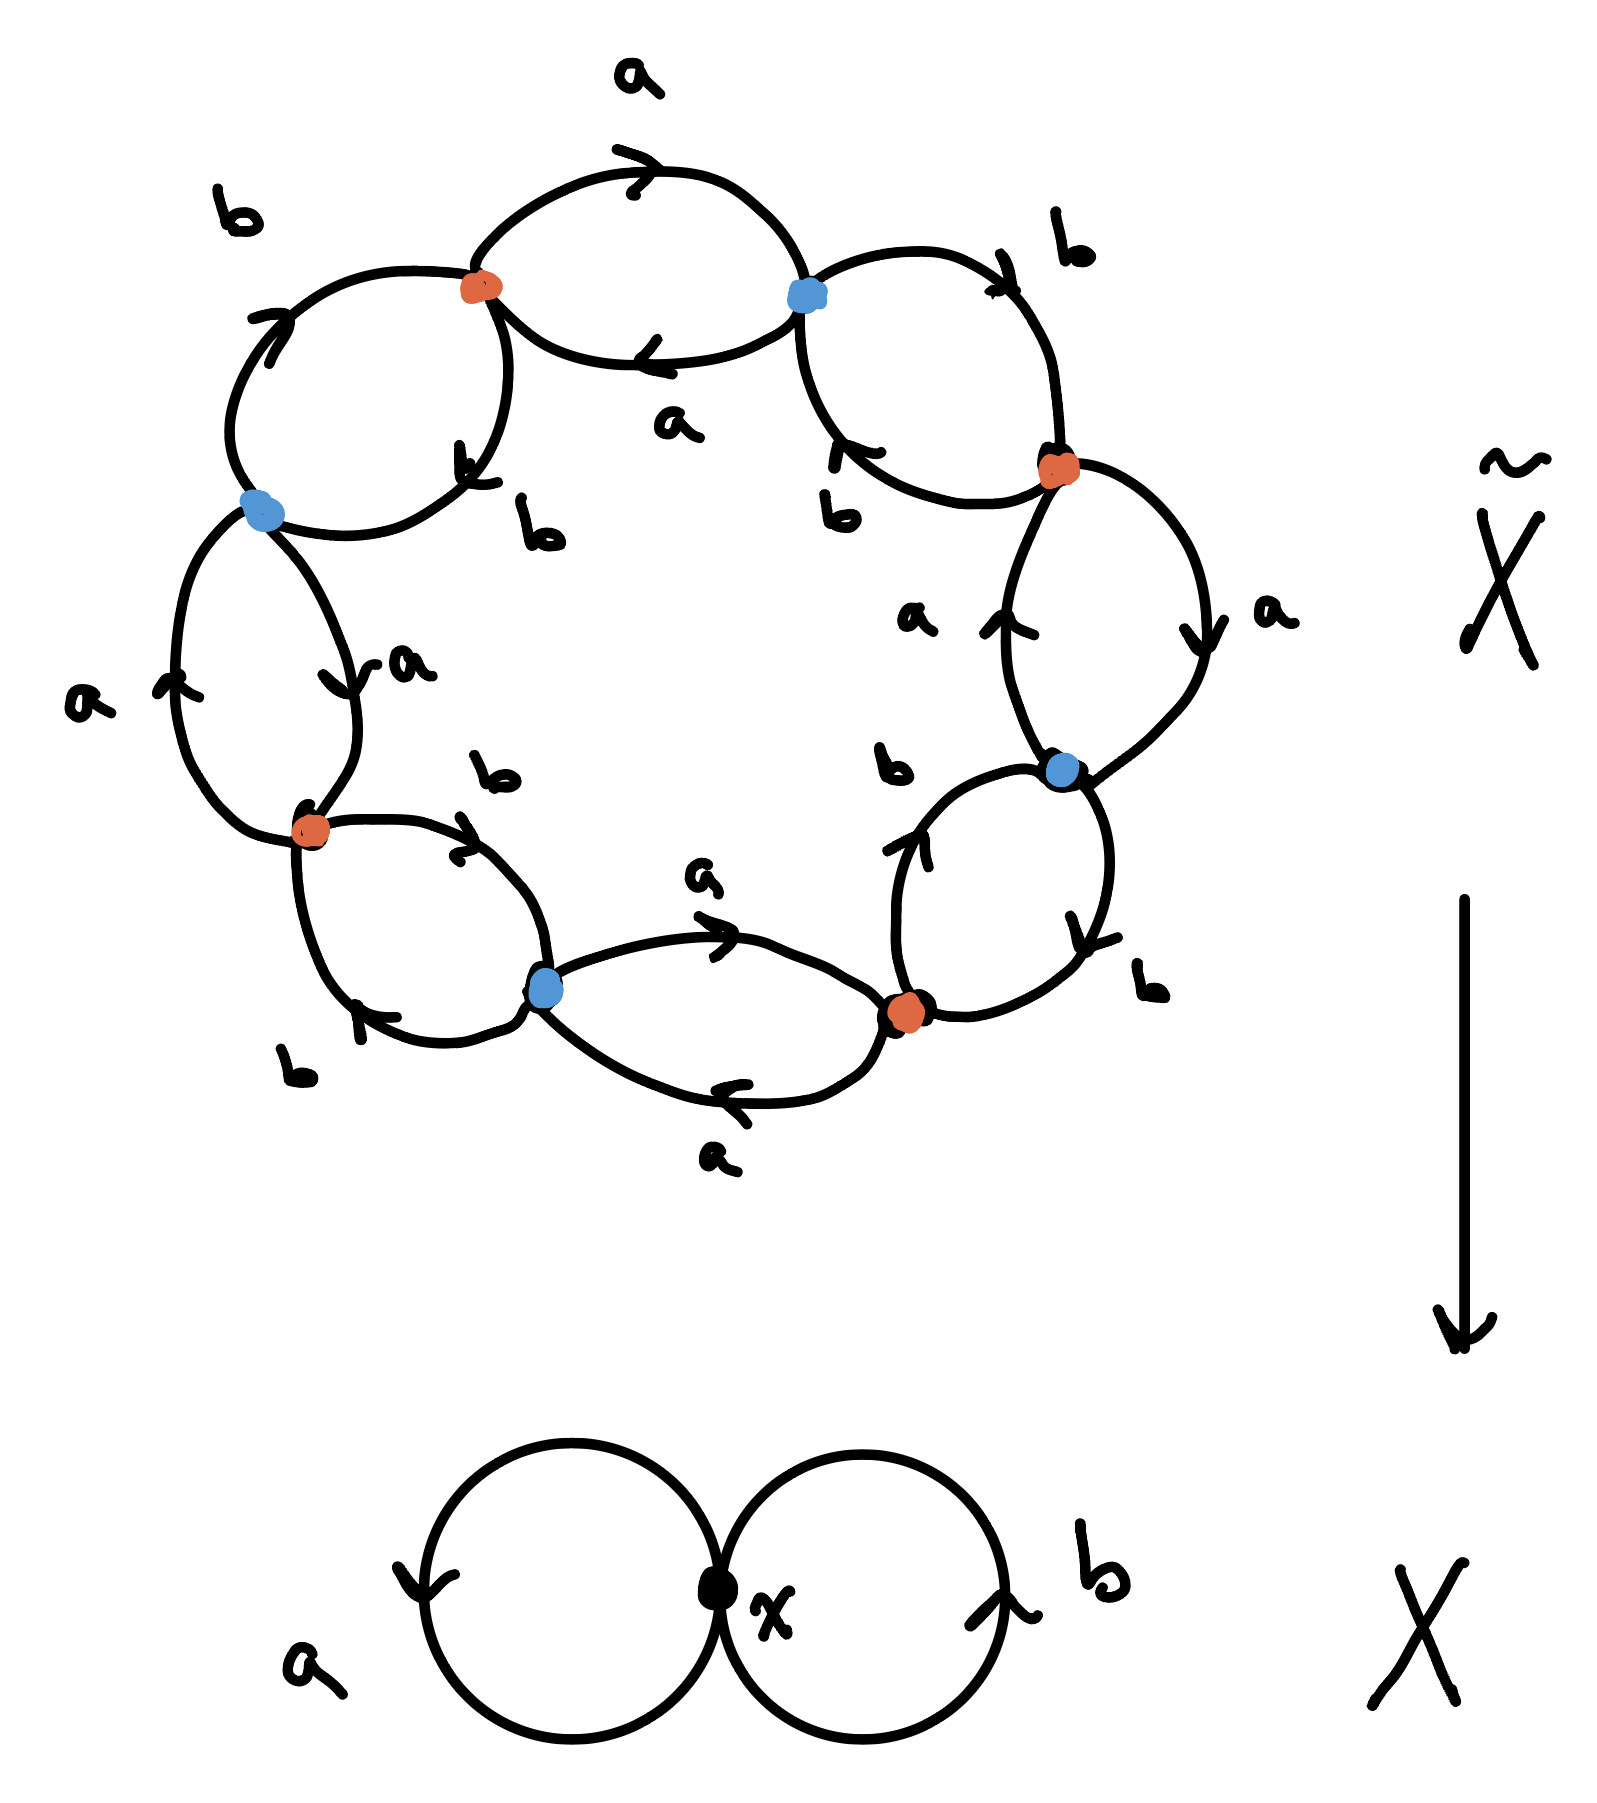
\includegraphics[width=10cm]{figures/hwk5-fig3.jpg}
      \captionof{figure}{Graph corresponding to $\langle a^2,b^2,(ab)^4 \rangle$.} 
      \label{fig:12_graph}
    \end{center}
  \end{prf}
  \prob[\textsc{Exercise 1.15}] Let $p:\tilX\to X$ be a simply-connected covering space of $X$ and let $A\subseteq X$ be a path-connected, locally path-connected subspace, with $\tilA\subseteq \tilX$ a path-component of $p^{-1}(A)$. Show that $p:\tilA\to A$ is the covering space corresponding to the kernel of the map $\pi_1(A)\to \pi_1(X)$.
  \begin{prf}
    Let $p' = p|_{\tilA}$ be the restriction of of $p$ to $\tilA$ with codomain $A$, $\iota:A\to X$ the inclusion of $A$ into $X$ and $\tilde{\iota}:\tilA\to \tilX$ the inclusion of $\tilA$ into $\tilX$. Note that we have $\iota \circ r = p\circ \tilde{\iota}$ by definition, and that the induced maps on fundamental groups satisfies the same relation.
    \begin{center}
      \begin{tikzcd}
        \tilA \arrow[r,"\tilde{\iota}"] \arrow[d,"r"] & \tilX \arrow[d,"p"] \\
        A \arrow[r,"\iota"] & X
      \end{tikzcd}
    \end{center}
    Since $X$ and $A$ are both path connected, we can choose $x_0$ to be the basepoint of each without this choice affecting their respective fundamental groups. Let $\tilx_0$ be the basepoint for $\tilA$ and $\tilX$ in the same way, such that $r(\tilx_0) = x_0$. With this notation in place, functoriality of the fundamental group gives us a corresponding commutative diagram:
    \begin{center}
      \begin{tikzcd}
        \pi_1(\tilA,\tilx_0) \arrow[r,"\tilde{\iota}_*"] \arrow[d,"r_*"] & \pi_1(\tilX,\tilx_0) \arrow[d,"p_*"] \\
        \pi_1(A,x_0) \arrow[r,"\iota_*"] & \pi_1(X,x_0)
      \end{tikzcd}.
    \end{center}
    
    I first claim that the map $r$ is a covering space of $A$. For each $x \in A$, take an evenly covered neighborhood $U$ of $x$ in $X$. Then $U\cap A$ is also an evenly covered neighborhood. Taking the preimage in $\tilX$ under $p$, intersecting with $\tilA$ and then taking the image under $r$ then gives us an evenly covered neighborhood of $x$ in $A$ whose preimage is entirely contained in $\tilA$.

    Now we want to show $p:\tilA\to A$ is the covering space of $A$ corresponding to the kernel of the map $\pi_1(A,x_0) \to \pi_1(X,x_0)$, or more precisely, that $r_*(\pi_1(\tilA,\tilx_0)) = \ker \iota_*$. Because $\tilX$ is simply-connected, $\pi_1(\tilX,\tilx_0) = 0$. The composition $p_*\circ \tilde{\iota}_*$ is therefore trivial, implying $\iota_* \circ r_* = 0$ too by the commutativity of the above diagram. This implies that $r_*(\pi_{1}(\tilA,x_0))\subseteq \ker \iota_*$.

    For the other inclusion, suppose we start with an element $[\gamma] \in \ker \iota_*$. This lifts to a unique path $\alpha$ in $\tilA$ with initial endpoint $\tilx_0$, and the composition of $\alpha$ with $\tilde{\iota}$ gives a path in $\tilX$. The commutativity of the first diagram means that $\tilde{\iota}\circ \alpha$ is a lift of $\iota\circ \gamma$, but this is homo topic to the trivial path at $x_0$ in $X$ since $[\gamma] \in \ker \iota_*$, hence $\tilde{\iota}\circ \alpha$ is actually a loop based at $x_0$. This means $\alpha$ is a loop in $\tilA$ and so $[\alpha]$ is an element $\pi_1(\tilA,\tilx_0)$. We know $[\gamma] = [r\circ \alpha]$ already since $\alpha$ was defined to be a lift of $\gamma$, hence $[\gamma] = r_*([\alpha])$. This gives us the other inclusion, and we are done.
  \end{prf}
  \prob[\textsc{Exercise 1.23}] Show that if a group $G$ acts freely and properly discontinuously on a Hausdorff space $X$, then the action is a covering space action. (Here ``properly discontinuously'' means that each $x \in X$ has a neighborhood $U$ such that $\{g \in G ~\mid~ U\cap g(U) \neq \emptyset\}$ is finite.) In particular, a free action of a finite group on a Hausdorff space is a covering space action.
  \begin{prf}
    Suppose that $G$ is a group which acts freely and properly discontinuously on a Hausdorff space $X$. For an open set $U\subseteq X$, define
    \begin{align*}
      S_U = \{g \in G~\mid~ U\cap g(U) \neq \emptyset\}.
    \end{align*}
    By the ``properly discontinuous'' hypothesis, we know that for each $x \in X$ we may find some open neighborhood $U_x$ such that $S_{U_x}$ is finite. We need only show that we can refine our choice of $U_x$ to guarantee $S_{U_x}$ is empty, as this is the definition of a covering space action.

    Fix $x \in X$ and $U_x$ as above, and enumerate $S_{U_x}$ as $\{g_1,...,g_n\}$ where $g_1 = e$. Because the action of $G$ is free, $g_ix = g_jx$ only if $i = j$. Using the Hausdorffness of $X$ we can therefore find an open neighborhood $V_i$ of $g_ix$ for each $1\leq i\leq n$ such that $V_i \cap V_j = \emptyset$ whenever $i\neq j$. Define $U = U_x \cap \bigcap_{i=1}^n g^{-1}_i(V_i)$. Each set $g^{-1}(V_i)$ contains $g^{-1}_ig_ix = x$ and is open, so $U$ is open and nonempty. Consider $U\cap g(U)$ for an arbitrary $g \in G$. If $g\not\in S_{U_x}$ then $U\cap g(U) \subseteq U_x\cap g(U_x) = \emptyset$, and if $g = g_i$ for some $1< i\leq n$, then
    \begin{align*}
      U \cap g(U) \subseteq g_1(g_1^{-1}(V_1)) \cap g_i(g_i^{-1}(V_i)) = V_1 \cap V_i = \emptyset.
    \end{align*}
    Thus, $U$ is an open neighborhood of $x$ such that $U\cap g(U) = \emptyset$ whenever $e \neq g \in G$, and hence the action of $G$ on $X$ is a covering space action.

    In particular, this means that every free action of a finite group on a Hausdorff space is a covering space action, since the action of a finite group on a topological space is automatically what Hatcher calls a ``properly discontinuous'' group action.
  \end{prf}
\end{homework}
\end{document}
